% ANGELEGT am 23.09.2026, Entscheidung des Verfassers: das Zeitmuster des
% Redispatch gehoert in den Anhang, damit Abschnitt 4.5 seine Aussagen
% belegen kann, ohne eine dreizehnte Abbildung ins Kapitel zu nehmen.
% Die Abbildung ist vom Analyse-Repository nach
% AUFTRAG_REDISPATCH_ZEITMUSTER.md geliefert und im Format der
% Abbildung 4.5 gesetzt. Die Zuordnung der Farben folgt den beiden
% Richtungen der kurativen Reservierung.
% Alle Zahlen stammen aus der eigenen Auswertung
% analysen/redispatch_tagesmuster und sind vom Analyse-Repository
% unabhaengig nachgerechnet und bestaetigt worden.
\chapter{Zeitmuster des Redispatch}
\label{anh:redispatch_zeitmuster}

In Abschnitt~\ref{sec:price_vs_redispatch} wird der kurative Reservierungspreis gegen den Engpassmanagementbedarf gehalten. Abbildung~\ref{fig:redispatch_zeitmuster} zeigt den Bedarf im selben Format wie Abbildung~\ref{fig:zeitmuster_reservierungspreis} den Preis, also über die Stunde des Tages und über den Monat. Grundlage sind die 19\,369 Einzelmaßnahmen des Jahres 2025, deren mittlere Leistung anteilig auf die berührten Stunden verteilt ist \cite{netztransparenz_regelenergie_2026}.

Die Zuordnung der Richtungen folgt der Wirkung eines Speichers. Soll die Einspeisung reduziert werden, so kann er statt einer Abregelung laden, was der Ladereservierung entspricht. Soll sie erhöht werden, so kann er entladen, was der Entladereservierung entspricht.

\begin{figure}[H]
    \centering
    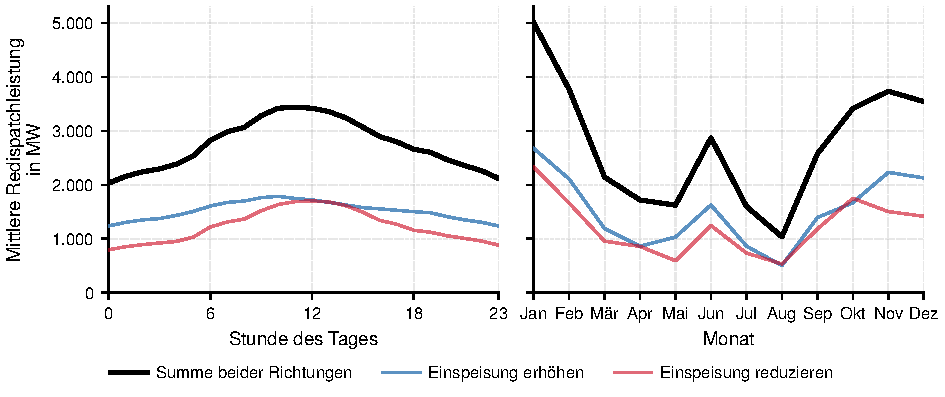
\includegraphics[width=\textwidth]{figures/anhang/redispatch_zeitmuster_2025.pdf}
    \caption{Mittlere Redispatchleistung des Jahres 2025 über die Stunde des Tages und über den Monat, je Richtung und als Summe.}
    \label{fig:redispatch_zeitmuster}
\end{figure}

Über den Tag schwankt die Summe beider Richtungen zwischen 2029 und 3440\,\si{MW}. Die Reduzierung der Einspeisung trägt das ausgeprägtere Muster, denn sie erreicht mittags mit 1701\,\si{MW} mehr als das Doppelte ihres nächtlichen Werts, während die Erhöhung um weniger als die Hälfte schwankt. Über das Jahr liegt der größte Monatswert im Januar mit 5010\,\si{MW} und der kleinste im August mit 1037\,\si{MW}.
